%%%%%%%%%%%%%%%%%%%%%%%%%%%%%%%%%%%%

\section{線形回帰における外れ値の種類}

%%%%%%%%%%%%%%%%%%%%%%%%%%%%%%%%%%%%

\begin{frame}
\frametitle{外れ値の種類}

\twocol{0.5}{0.5}
{
\dq{この散布図において、外れ値は最小二乗直線にどのような影響を与えているか？}

この問いに答えるために、外れ値がある場合とない場合の回帰直線がどうなるかを考える。外れ値がない場合、回帰直線はより急な傾きになり、大きな観測値の集まりに近くなる。外れ値がある場合、直線は上方に引っ張られ、大きな観測値の集まりの一部から遠ざかる。
}
{
\begin{center}
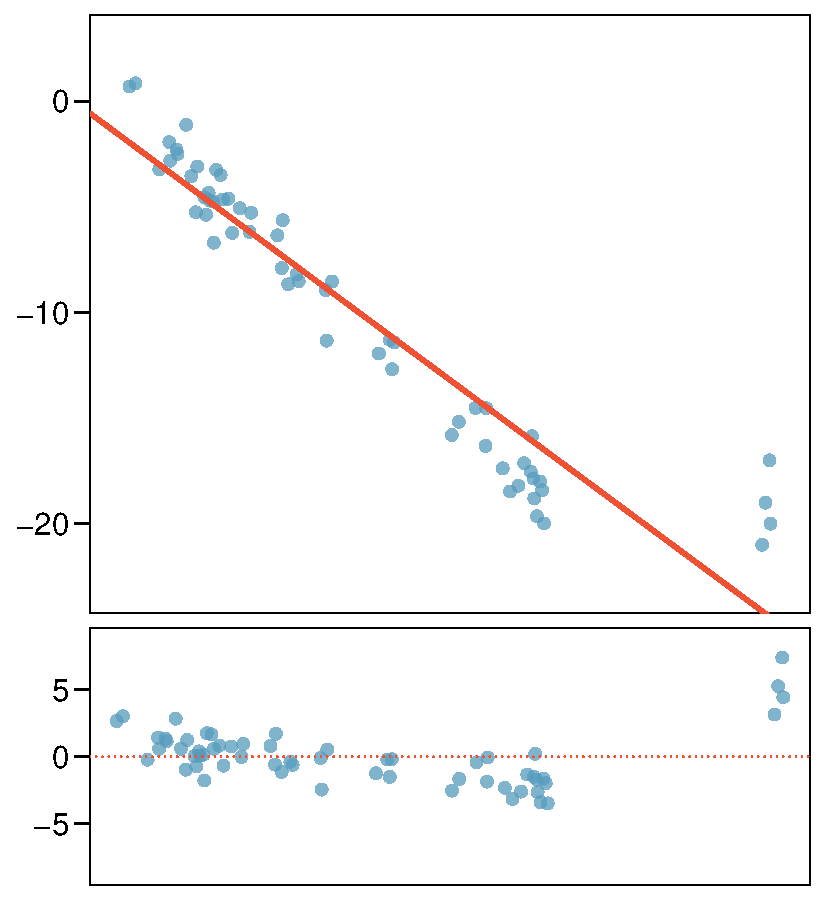
\includegraphics[width=\textwidth]{8-3_outliers/figures/outlierPlots/out4}
\end{center}
}

\end{frame}

%%%%%%%%%%%%%%%%%%%%%%%%%%%%%%%%%%%

\begin{frame}
\frametitle{外れ値の種類}

\twocol{0.4}{0.6}
{
\dq{この散布図において、外れ値は最小二乗直線にどのような影響を与えているか？} \\
\soln{外れ値がない場合、$x$と$y$の間に明らかな関係は見られない。}
}
{
\begin{center}
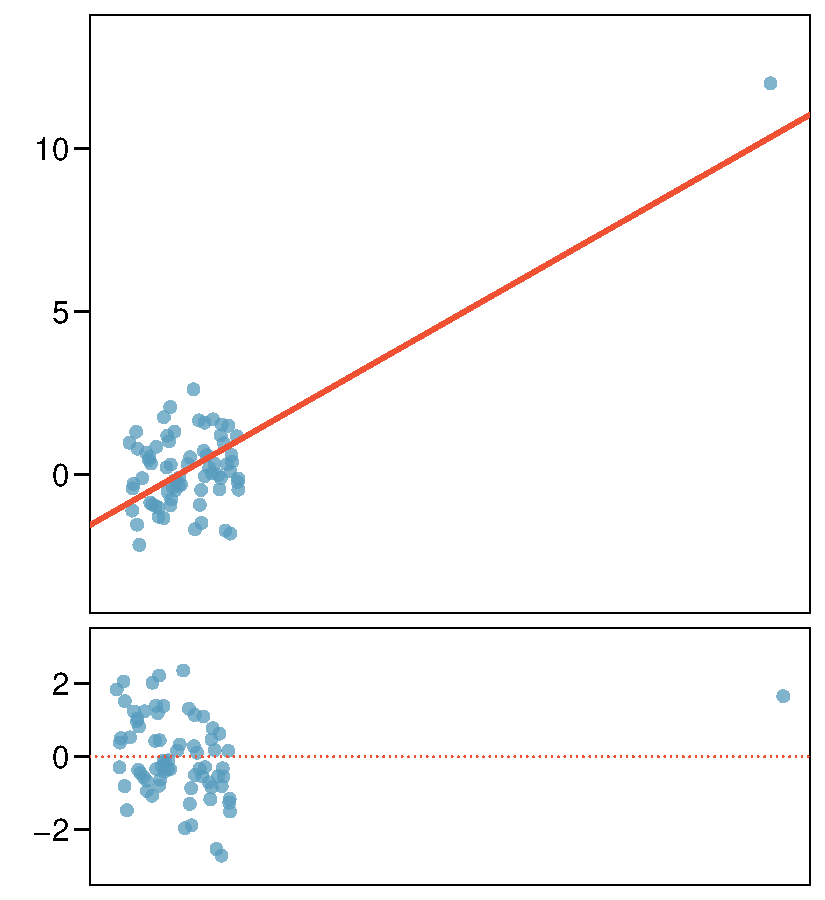
\includegraphics[width=\textwidth]{8-3_outliers/figures/outlierPlots/out5}
\end{center}
}

\end{frame}

%%%%%%%%%%%%%%%%%%%%%%%%%%%%%%%%%%%

\begin{frame}
\frametitle{用語}

\begin{itemize}

\item \hl{外れ値}とは、点の集まりから離れた位置にある点のことである。

\item 点の集まりの中心から水平方向に離れた外れ値を\hl{高レバレッジ点}（high leverage points）と呼ぶ。

\item 回帰直線の\underline{傾き}に実際に影響を与える高レバレッジ点を\hl{影響点}（influential points）と呼ぶ。

\item ある点が影響点かどうかを判断するには、その点がある場合とない場合の回帰直線を視覚的に比較する。直線の傾きが大きく変わる場合、その点は影響点である。大きく変わらない場合は影響点ではない。

\end{itemize}

\end{frame}

%%%%%%%%%%%%%%%%%%%%%%%%%%%%%%%%%%%

\begin{frame}
\frametitle{影響点}

星団CYG OB1に属する47個の星について、表面温度の対数と光度の対数のデータが得られている。

\twocol{0.7}{0.3}
{
\begin{center}
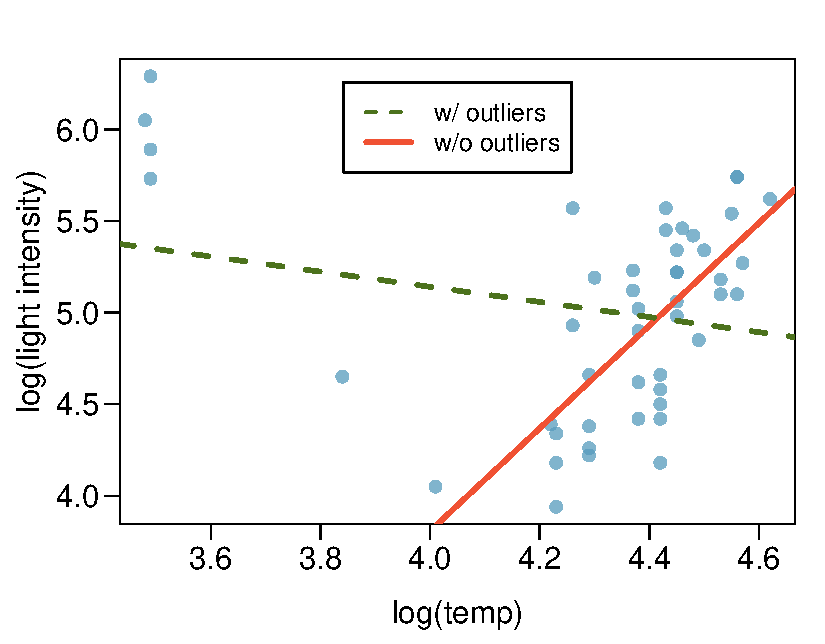
\includegraphics[width=\textwidth]{8-3_outliers/figures/stars/star}
\end{center}
}
{
\begin{center}
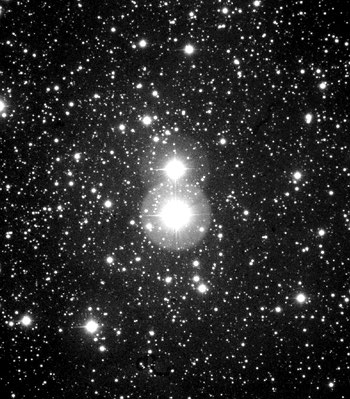
\includegraphics[width=\textwidth]{8-3_outliers/figures/stars/cyg}
\end{center}
}

\end{frame}

%%%%%%%%%%%%%%%%%%%%%%%%%%%%%%%%%%%

\begin{frame}
\frametitle{外れ値の種類}

\twocol{0.4}{0.6}
{
\pq{この外れ値を最もよく表す記述はどれか？}
\begin{enumerate}[(a)]
\item 影響点
\solnMult{高レバレッジ点}
\item 上記のいずれでもない
\item 外れ値はない
\end{enumerate}
}
{
\begin{center}
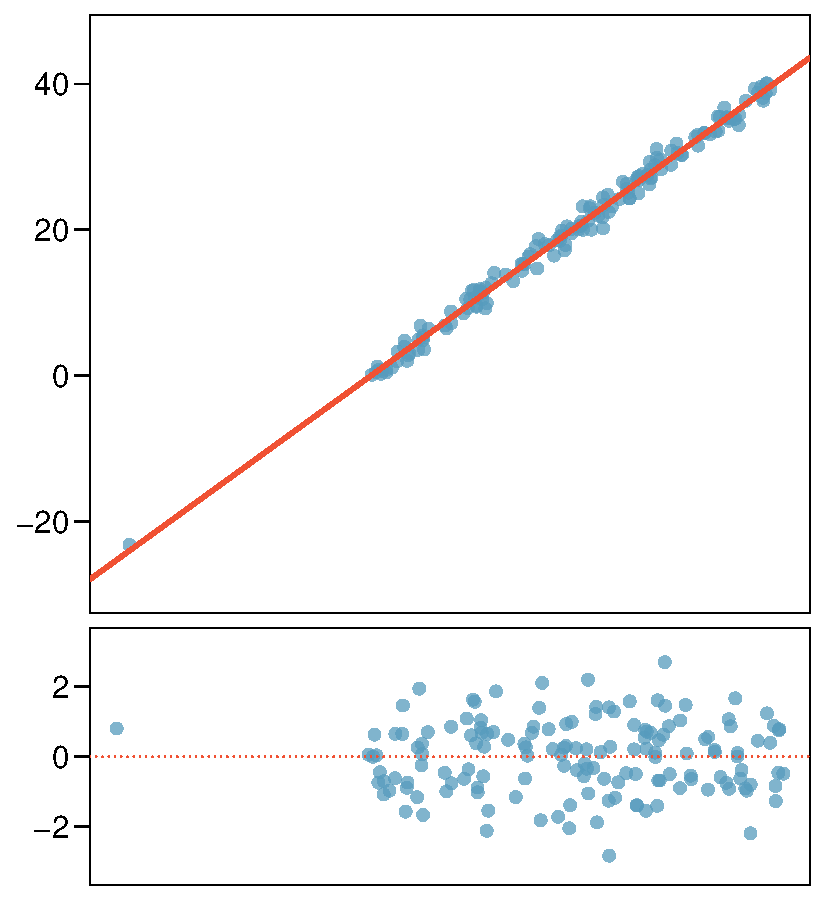
\includegraphics[width=\textwidth]{8-3_outliers/figures/outlierPlots/out6}
\end{center}
}

\end{frame}

%%%%%%%%%%%%%%%%%%%%%%%%%%%%%%%%%%%

\begin{frame}
\frametitle{外れ値の種類}

\twocol{0.4}{0.6}
{
\dq{この外れ値は回帰直線の傾きに影響を与えているか？}
\soln{あまり影響していない…}

}
{
\begin{center}
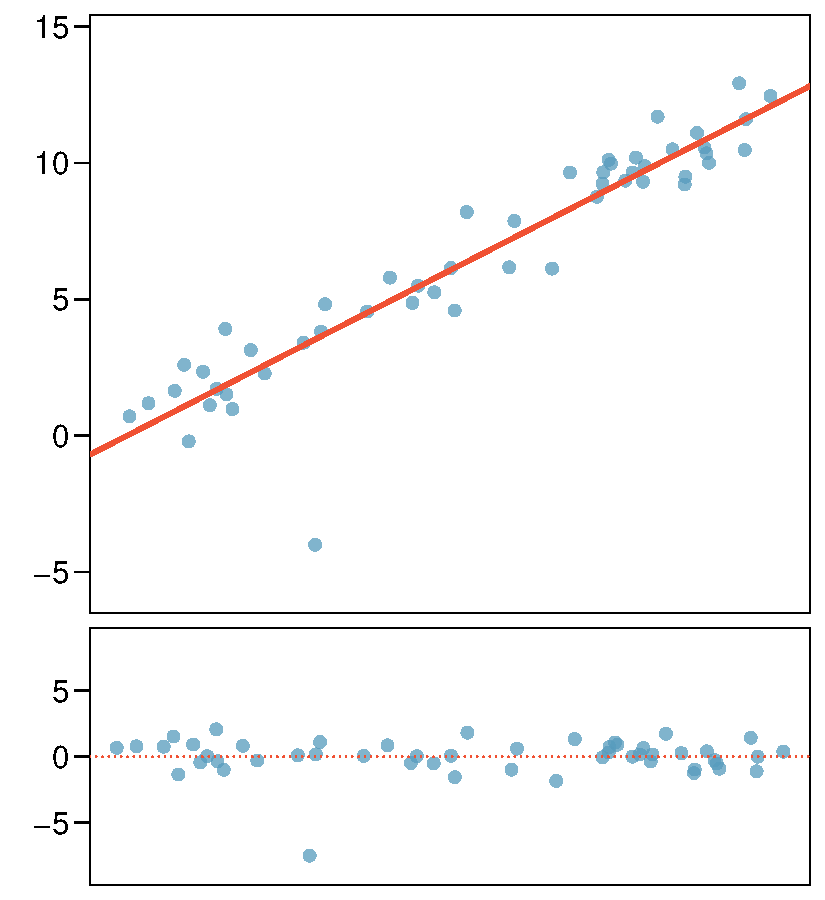
\includegraphics[width=\textwidth]{8-3_outliers/figures/outlierPlots/out1}
\end{center}
}

\end{frame}

%%%%%%%%%%%%%%%%%%%%%%%%%%%%%%%%%%%

\begin{frame}
\frametitle{まとめ}

\pq{次のうち\underline{正しい}記述はどれか？}

\begin{enumerate}[(a)]
\item 影響点は常に回帰直線の切片を変化させる。
\item 影響点は常に$R^2$を低下させる。
\item 低レバレッジ点の方が高レバレッジ点よりも影響点になりやすい。
\item データセットに影響点が含まれる場合、説明変数と目的変数の関係は常に非線形である。
\solnMult{上記のいずれも正しくない。}
\end{enumerate}

\end{frame}

%%%%%%%%%%%%%%%%%%%%%%%%%%%%%%%%%%%

\begin{frame}
\frametitle{まとめ（続き）}

\vspace{-1cm}

\twocol{0.5}{0.5}
{
\begin{center}
\[ R = 0.08, R^2 = 0.0064 \]
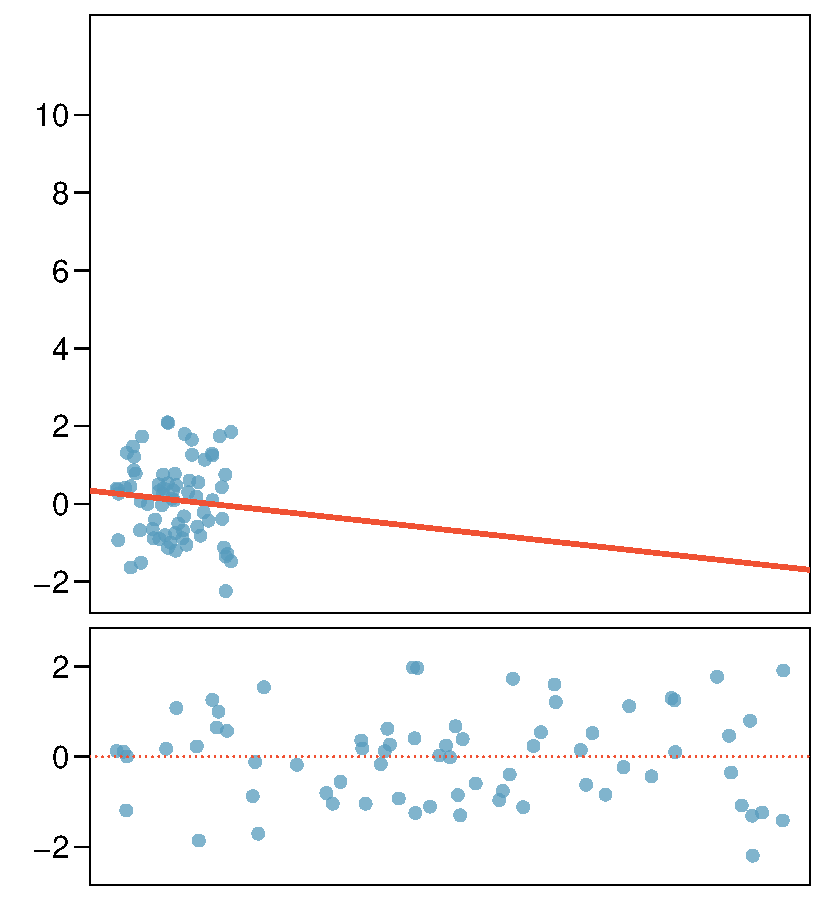
\includegraphics[width=\textwidth]{8-3_outliers/figures/outlierPlots/out5-1}
\end{center}
}
{
\begin{center}
\[ R = 0.79, R^2 = 0.6241 \]
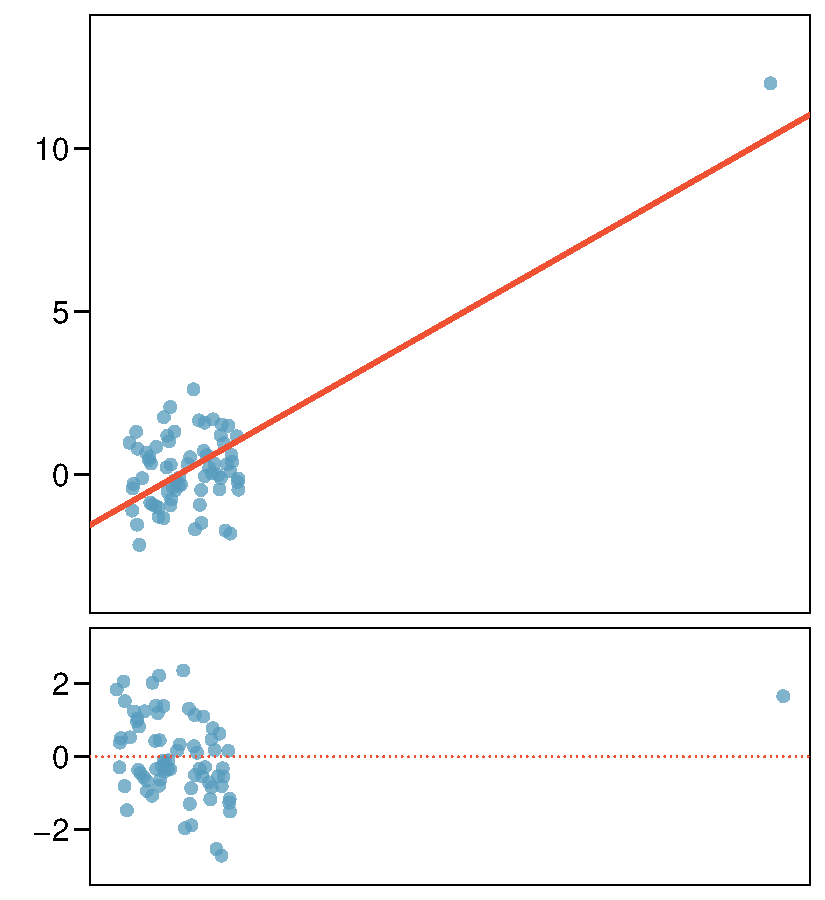
\includegraphics[width=\textwidth]{8-3_outliers/figures/outlierPlots/out5}
\end{center}
}

\end{frame}
